\subsection{Betriebssystem starten}
Beim ersten Start des Raspberry öffnet sich nach kurzer Wartezeit ein graues Fenster auf blauem Hintergrund mit dem Titel ``Raspberry Pi Software Configuration Tool". 

\begin{figure}[h]
\centering
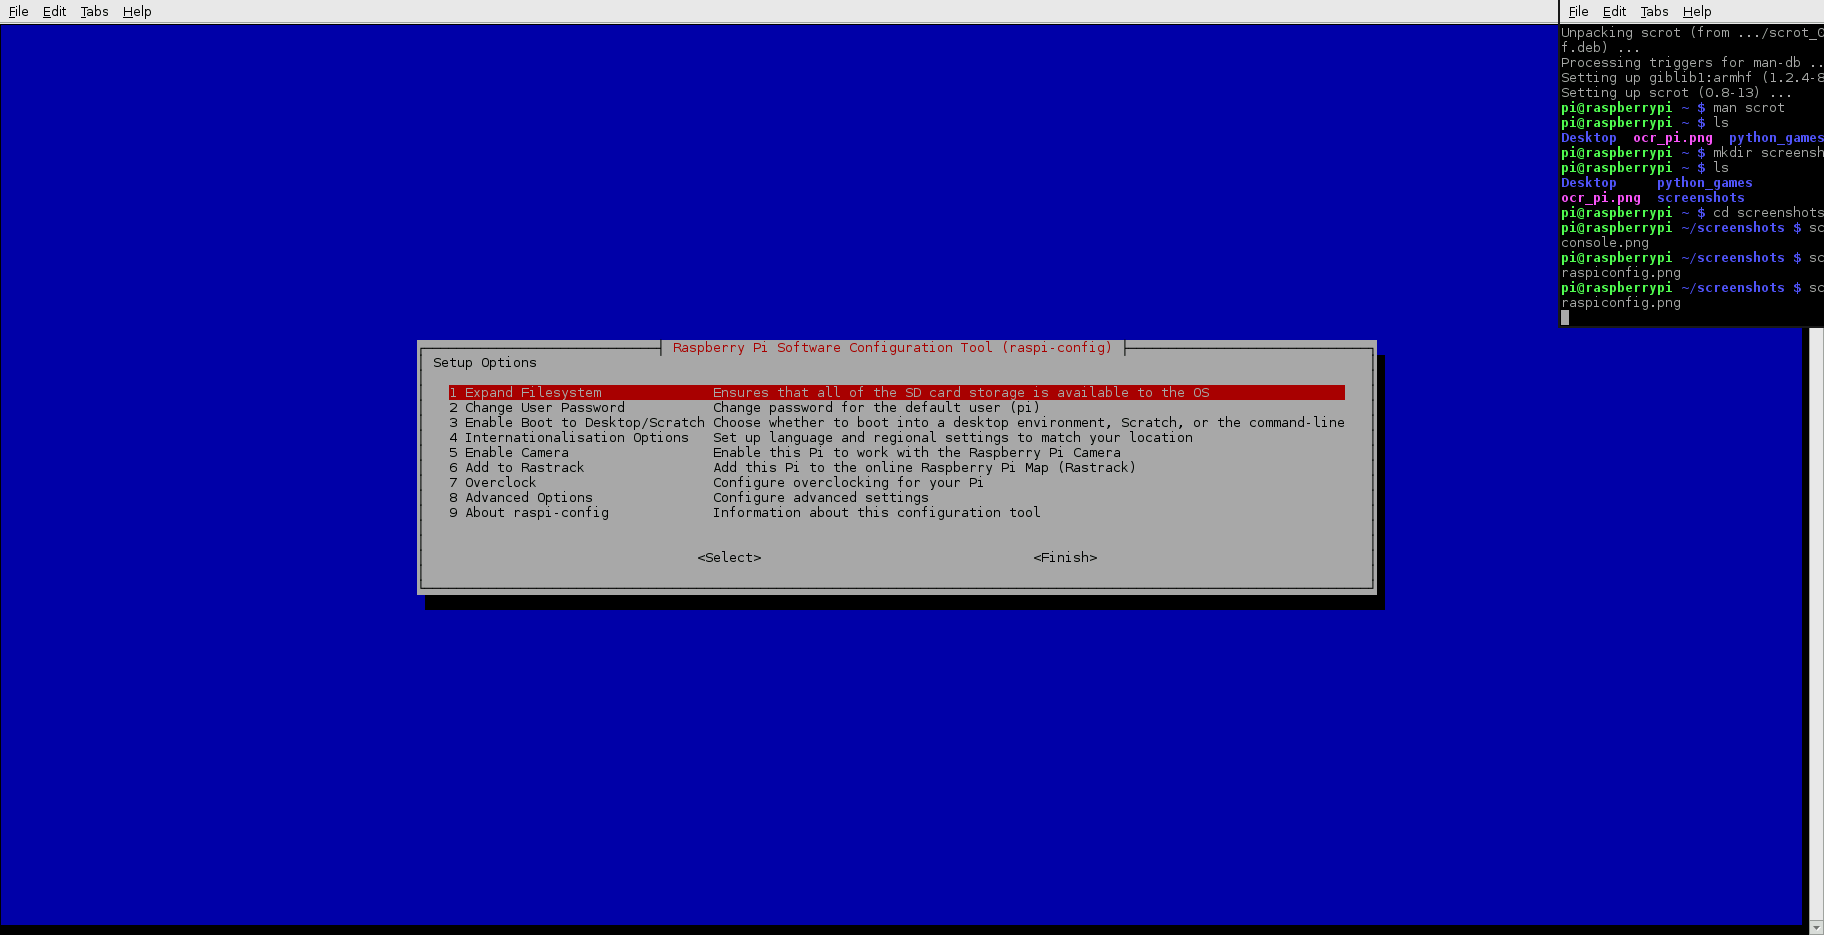
\includegraphics[scale=0.5]{../images/raspiconfig}
\caption{Raspberry Pi Konfigurations-Tool}
\end{figure}

Dieses Werkzeug dient dazu, gewisse Grundeinstellungen vorzunehmen. Folgende Einstellungen sollten vorgenommen werden: 

\begin{enumerate}
\item Benutzerpasswort ändern (Change User Password)
\item Ausweiten des Dateisystems, um den Speicher der Karte voll auszunutzen (Expand Filesystem)
\item Anpassen des Keyboardlayouts (Internationalisation Options > Change Keyboard Layout)
\item Regionaleinstellungen auf en\_US.UTF-8 setzen (Internationalisation Options > Change Locale)
\item Zeitregion setzen (Internationalisation Options > Change Timezone) 
\item Raspberry Pi übertakten auf "Medium, 900MHz" (Overclock)
\item Speicherverteilung für die GPU auf 16 (Megabyte, MB) begrenzen (Advanced Options > A3 Memory Split)
\end{enumerate}

Sollte es mit den getroffenen Einstellungen zu Problemen kommen, kann das Konfigurationstool im laufenden Betrieb erneut aufgerufen werden. Folgender Befehl muss dazu in der Konsole eingegeben werden: 

\begin{lstlisting}
sudo raspi-config
\end{lstlisting} 

Sind alle Einstellungen vorgenommen, kann das Menü mittels ``Finish" verlassen werden. Die Frage, ob neu gestartet werden soll (reboot), mit "Ja" beantworten, worauf das System neu startet und alle zuvor vorgenommenen Einstellungen übernommen werden.
\\
\\
Nach dem Neustart findet man sich in einem konsolenartigen Fenster mit einem blinkenden Cursor wieder. Dies wird für den Rest des Tutorials die Arbeitsumgebung sein, da die grafische Benutzeroberfläche nicht gebraucht wird. Die Performance ist in der Konsole zudem deutlich besser.

\subsection{Root-Rechte erlangen}
Die meisten der in dieser Anleitung beschriebenen Befehle verlangen erweiterte Rechte. Diese können unter Raspbian ganz einfach erlangt werden mittels:

\begin{lstlisting}
sudo su
\end{lstlisting}

Grosse Macht bringt auch grosse Verantwortung. Hat man unter Linux Administrator-Rechte (auch Root-Rechte genannt), kann man sehr schnell sehr vieles kaputt machen. Im schlimmsten Fall muss die SD-Karte neu aufgesetzt werden. Es lohnt sich deshalb, ein paar wenige Regeln zum Gebrauch der Konsole zu beachten: 

\begin{itemize}
\item Ein Befehl wird mittels Drücken der ``Enter-Taste" abgesetzt
\item Bevor ein neuer Befehl abgsetzt werden, muss der zuvor eingegebene abgeschlossen sein (manchmal ist Geduld gefragt)
\item Gross- und Kleinschreibung werden unter Linux unterschieden!
\item Immer sicherstellen, dass der Befehl auch wirklich richtig eingegeben wurde
\end{itemize}

Als Root-User sollte man nur dann unterwegs sein, wenn man die erweiterten Rechte für einen längeren Zeitraum benötigt, wie das in diesem Tutorial der Fall ist. Für einzelne Befehle kann auch \textit{sudo} verwendet werden. Dieses Schlüsselwort wird einfach jedem Befehl vorangestellt, der erweiterte Rechte verlangt.
\\
Ein Beispiel:

\begin{lstlisting}
sudo apt-get update
\end{lstlisting}

Am Ende dieses Tutorials sollten die Root-Rechte unbedingt wieder abgegeben werden. Um das zu tun, reicht ein einfaches \textit{exit} in der Kommandozeile und schon ist man wieder als normaler User unterwegs.

\subsection{System aktualisieren}
Um sicherzustellen, dass das System auf dem aktuellsten Stand ist, müssen zuerst alle installierten Pakete aktualisiert werden. Dazu müssen folgende zwei Befehle abgesetzt werden:

\begin{lstlisting}
apt-get update
apt-get upgrade
\end{lstlisting}

Nach der Eingabe von \textit{apt-get upgrade} fragt das Terminal noch einmal nach, ob man die zur Verfügung stehenden Pakete wirklich installieren will. Standardmässig ist die Antwort auf \textit{Ja} eingestellt, was man an dem grossen Y in \textit{[Y/n]} erkennt. Um fortzufahren reicht ein erneutes Drücken der Enter-Taste. Zukünftige Rückfragen bei abgesetzten Befehlen können auf die gleiche Weise behandelt werden. Es empfiehlt sich dennoch, die angezeigte Meldungen (Informationen, Warnungen) immer durchzulesen und entsprechend zu handeln.

\begin{figure}[h]
\centering
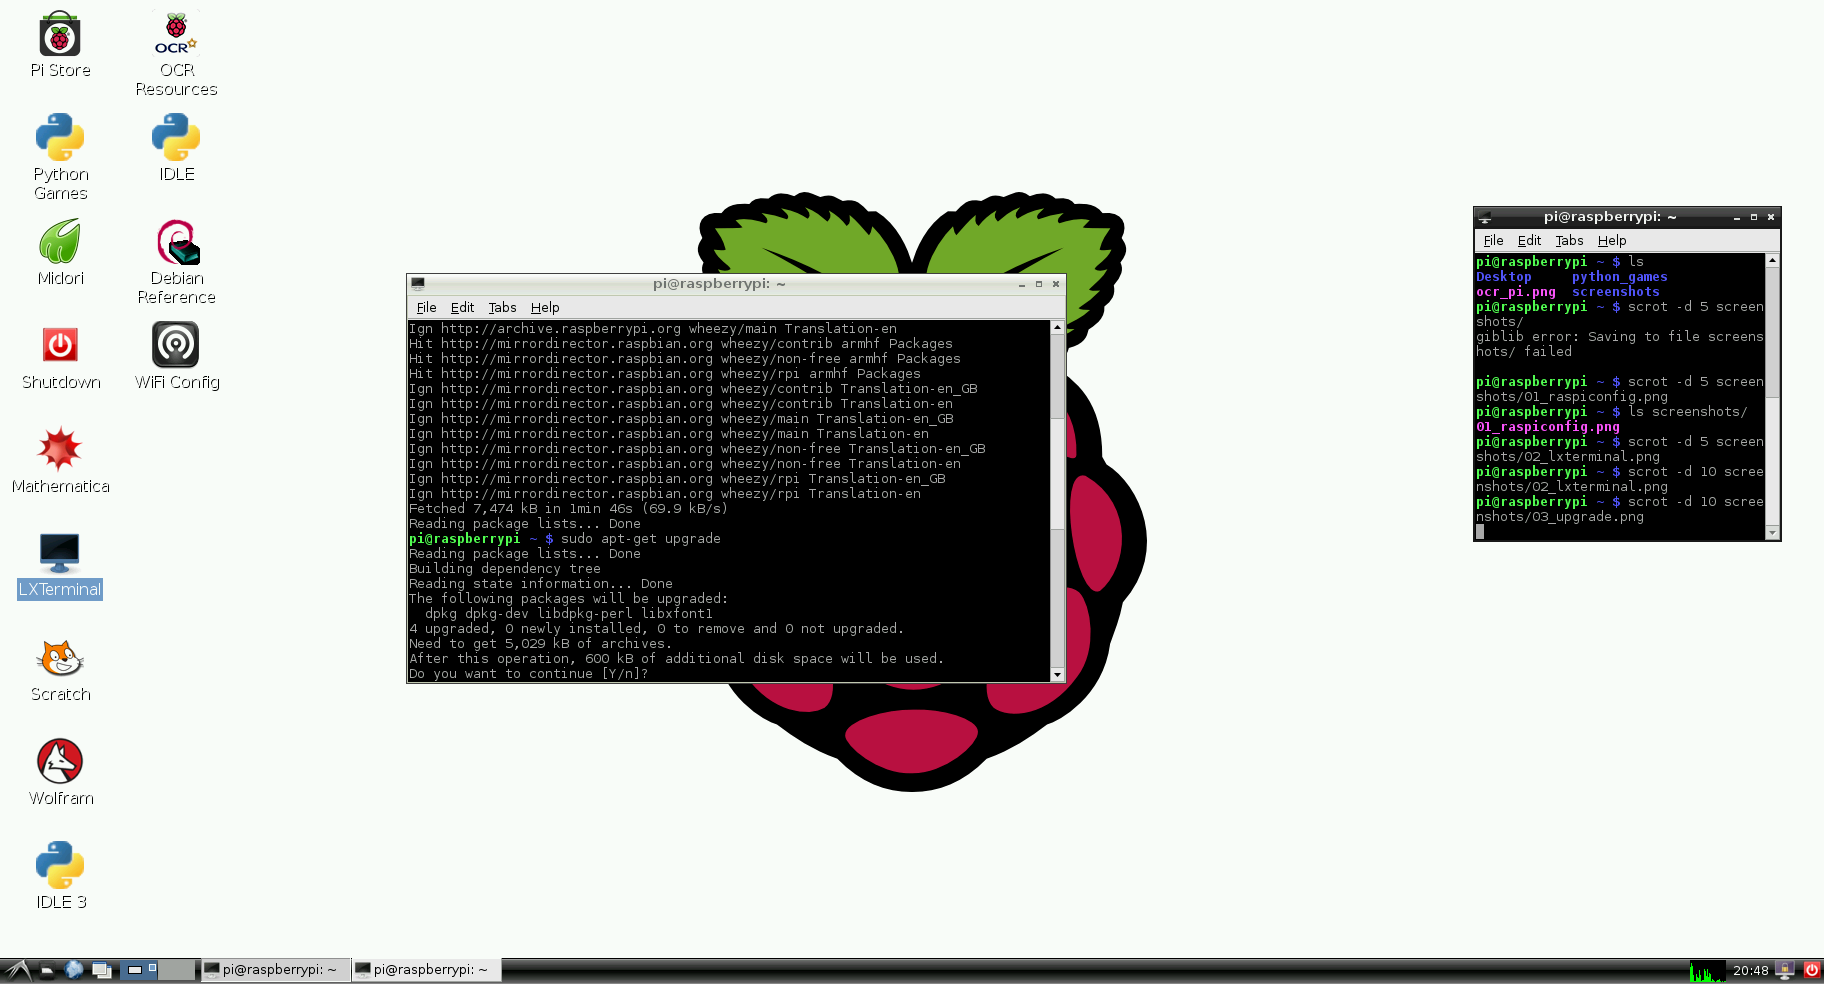
\includegraphics[scale=0.7]{../images/upgrade}
\caption{apt-get upgrade}
\end{figure}
